% Options for packages loaded elsewhere
\PassOptionsToPackage{unicode}{hyperref}
\PassOptionsToPackage{hyphens}{url}
\PassOptionsToPackage{dvipsnames,svgnames,x11names}{xcolor}
%
\documentclass[
]{article}

\usepackage{amsmath,amssymb}
\usepackage{iftex}
\ifPDFTeX
  \usepackage[T1]{fontenc}
  \usepackage[utf8]{inputenc}
  \usepackage{textcomp} % provide euro and other symbols
\else % if luatex or xetex
  \usepackage{unicode-math}
  \defaultfontfeatures{Scale=MatchLowercase}
  \defaultfontfeatures[\rmfamily]{Ligatures=TeX,Scale=1}
\fi
\usepackage{lmodern}
\ifPDFTeX\else  
    % xetex/luatex font selection
\fi
% Use upquote if available, for straight quotes in verbatim environments
\IfFileExists{upquote.sty}{\usepackage{upquote}}{}
\IfFileExists{microtype.sty}{% use microtype if available
  \usepackage[]{microtype}
  \UseMicrotypeSet[protrusion]{basicmath} % disable protrusion for tt fonts
}{}
\makeatletter
\@ifundefined{KOMAClassName}{% if non-KOMA class
  \IfFileExists{parskip.sty}{%
    \usepackage{parskip}
  }{% else
    \setlength{\parindent}{0pt}
    \setlength{\parskip}{6pt plus 2pt minus 1pt}}
}{% if KOMA class
  \KOMAoptions{parskip=half}}
\makeatother
\usepackage{xcolor}
\setlength{\emergencystretch}{3em} % prevent overfull lines
\setcounter{secnumdepth}{-\maxdimen} % remove section numbering
% Make \paragraph and \subparagraph free-standing
\makeatletter
\ifx\paragraph\undefined\else
  \let\oldparagraph\paragraph
  \renewcommand{\paragraph}{
    \@ifstar
      \xxxParagraphStar
      \xxxParagraphNoStar
  }
  \newcommand{\xxxParagraphStar}[1]{\oldparagraph*{#1}\mbox{}}
  \newcommand{\xxxParagraphNoStar}[1]{\oldparagraph{#1}\mbox{}}
\fi
\ifx\subparagraph\undefined\else
  \let\oldsubparagraph\subparagraph
  \renewcommand{\subparagraph}{
    \@ifstar
      \xxxSubParagraphStar
      \xxxSubParagraphNoStar
  }
  \newcommand{\xxxSubParagraphStar}[1]{\oldsubparagraph*{#1}\mbox{}}
  \newcommand{\xxxSubParagraphNoStar}[1]{\oldsubparagraph{#1}\mbox{}}
\fi
\makeatother


\providecommand{\tightlist}{%
  \setlength{\itemsep}{0pt}\setlength{\parskip}{0pt}}\usepackage{longtable,booktabs,array}
\usepackage{calc} % for calculating minipage widths
% Correct order of tables after \paragraph or \subparagraph
\usepackage{etoolbox}
\makeatletter
\patchcmd\longtable{\par}{\if@noskipsec\mbox{}\fi\par}{}{}
\makeatother
% Allow footnotes in longtable head/foot
\IfFileExists{footnotehyper.sty}{\usepackage{footnotehyper}}{\usepackage{footnote}}
\makesavenoteenv{longtable}
\usepackage{graphicx}
\makeatletter
\newsavebox\pandoc@box
\newcommand*\pandocbounded[1]{% scales image to fit in text height/width
  \sbox\pandoc@box{#1}%
  \Gscale@div\@tempa{\textheight}{\dimexpr\ht\pandoc@box+\dp\pandoc@box\relax}%
  \Gscale@div\@tempb{\linewidth}{\wd\pandoc@box}%
  \ifdim\@tempb\p@<\@tempa\p@\let\@tempa\@tempb\fi% select the smaller of both
  \ifdim\@tempa\p@<\p@\scalebox{\@tempa}{\usebox\pandoc@box}%
  \else\usebox{\pandoc@box}%
  \fi%
}
% Set default figure placement to htbp
\def\fps@figure{htbp}
\makeatother

% Cấu hình font chữ chính và toán học
\usepackage{fontspec}
\usepackage{unicode-math}
\setmainfont{STIX Two Text}
\setsansfont{STIX Two Text}
\setmonofont{STIX Two Text}
\setmathfont{STIX Two Math}

% Cấu hình kích thước chữ
% \fontsize{12pt}{14pt}\selectfont

% Đánh số section
\setcounter{secnumdepth}{3}

% Các gói hỗ trợ bổ sung
\usepackage{hyperref}  % Hỗ trợ liên kết
\usepackage{graphicx}  % Hỗ trợ hình ảnh
\usepackage{amsmath, amssymb}  % Hỗ trợ toán học nâng cao
\usepackage{svg}  % Hỗ trợ hình ảnh SVG
\usepackage{xcolor}
\usepackage{tikz}
  \usetikzlibrary{arrows, positioning}
\makeatletter
\@ifpackageloaded{tcolorbox}{}{\usepackage[skins,breakable]{tcolorbox}}
\@ifpackageloaded{fontawesome5}{}{\usepackage{fontawesome5}}
\definecolor{quarto-callout-color}{HTML}{909090}
\definecolor{quarto-callout-note-color}{HTML}{0758E5}
\definecolor{quarto-callout-important-color}{HTML}{CC1914}
\definecolor{quarto-callout-warning-color}{HTML}{EB9113}
\definecolor{quarto-callout-tip-color}{HTML}{00A047}
\definecolor{quarto-callout-caution-color}{HTML}{FC5300}
\definecolor{quarto-callout-color-frame}{HTML}{acacac}
\definecolor{quarto-callout-note-color-frame}{HTML}{4582ec}
\definecolor{quarto-callout-important-color-frame}{HTML}{d9534f}
\definecolor{quarto-callout-warning-color-frame}{HTML}{f0ad4e}
\definecolor{quarto-callout-tip-color-frame}{HTML}{02b875}
\definecolor{quarto-callout-caution-color-frame}{HTML}{fd7e14}
\makeatother
\makeatletter
\@ifpackageloaded{caption}{}{\usepackage{caption}}
\AtBeginDocument{%
\ifdefined\contentsname
  \renewcommand*\contentsname{Mục lục}
\else
  \newcommand\contentsname{Mục lục}
\fi
\ifdefined\listfigurename
  \renewcommand*\listfigurename{Danh sách hình}
\else
  \newcommand\listfigurename{Danh sách hình}
\fi
\ifdefined\listtablename
  \renewcommand*\listtablename{Danh sách bảng}
\else
  \newcommand\listtablename{Danh sách bảng}
\fi
\ifdefined\figurename
  \renewcommand*\figurename{Hình}
\else
  \newcommand\figurename{Hình}
\fi
\ifdefined\tablename
  \renewcommand*\tablename{Bảng}
\else
  \newcommand\tablename{Bảng}
\fi
}
\@ifpackageloaded{float}{}{\usepackage{float}}
\floatstyle{ruled}
\@ifundefined{c@chapter}{\newfloat{codelisting}{h}{lop}}{\newfloat{codelisting}{h}{lop}[chapter]}
\floatname{codelisting}{Listing}
\newcommand*\listoflistings{\listof{codelisting}{List of Listings}}
\makeatother
\makeatletter
\makeatother
\makeatletter
\@ifpackageloaded{caption}{}{\usepackage{caption}}
\@ifpackageloaded{subcaption}{}{\usepackage{subcaption}}
\makeatother
\makeatletter
\@ifpackageloaded{sidenotes}{}{\usepackage{sidenotes}}
\@ifpackageloaded{marginnote}{}{\usepackage{marginnote}}
\makeatother

\ifLuaTeX
\usepackage[bidi=basic]{babel}
\else
\usepackage[bidi=default]{babel}
\fi
\babelprovide[main,import]{vietnamese}
% get rid of language-specific shorthands (see #6817):
\let\LanguageShortHands\languageshorthands
\def\languageshorthands#1{}
\usepackage{bookmark}

\IfFileExists{xurl.sty}{\usepackage{xurl}}{} % add URL line breaks if available
\urlstyle{same} % disable monospaced font for URLs
\hypersetup{
  pdftitle={Bài 1. Tính đơn điệu và cực trị của hàm số},
  pdfauthor={ZO Math},
  pdflang={vi},
  colorlinks=true,
  linkcolor={blue},
  filecolor={Maroon},
  citecolor={Blue},
  urlcolor={Blue},
  pdfcreator={LaTeX via pandoc}}


\title{Bài 1. Tính đơn điệu và cực trị của hàm số}
\usepackage{etoolbox}
\makeatletter
\providecommand{\subtitle}[1]{% add subtitle to \maketitle
  \apptocmd{\@title}{\par {\large #1 \par}}{}{}
}
\makeatother
\subtitle{Chương 1 \textbar{} Chân Trời Sáng Tạo \textbar{} Toán 12}
\author{ZO Math}
\date{13-04-2025}

\begin{document}
\maketitle


Hoạt động khởi động

\begin{figure}

\begin{minipage}{0.50\linewidth}
Trong 8 phút đầu kể từ khi xuất phát, độ cao \(h\) (tính bằng mét) của
khinh khí cầu vào thời điểm \(t\) phút được cho bởi công thức
\(h(t) = 6t^3 − 81t^2 + 324t\). Đồ thị của hàm số \(h(t)\) được biểu
diễn trong hình bên. Trong các khoảng thời gian nào khinh khí cầu tăng
dần độ cao, giảm dần độ cao? Độ cao của khinh khí cầu vào các thời điểm
3 phút và 6 phút sau khi xuất phát có gì đặc biệt?\end{minipage}%
%
\begin{minipage}{0.50\linewidth}
\hfill
\pandocbounded{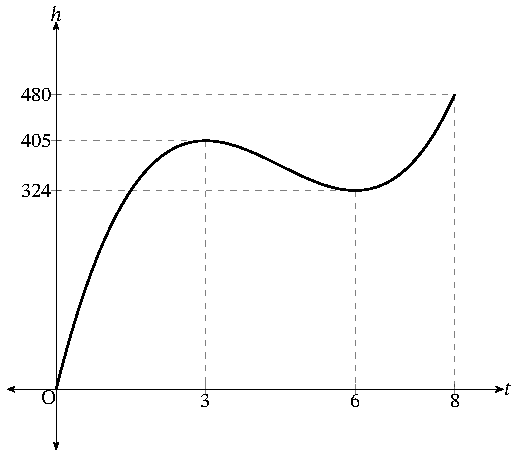
\includegraphics[keepaspectratio]{../../../../../../../figures/toan-thpt/toan-12/chan-troi/sach-giao-khoa/chuong-1/bai-1/hoat-dong-khoi-dong.pdf}}\end{minipage}%

\end{figure}%

Luận giải: Bóng tối

Có những đồ thị không chỉ uốn lượn theo trục tọa độ, mà còn lặng lẽ vẽ
nên những chuyển động khiến lòng người nao nao. Không cần lời giải,
không cần định lý - chỉ cần ngắm nhìn đường cong ấy thôi cũng đủ thấy
tim mình bị kéo theo từng nhịp lên xuống. Khởi đầu nhẹ như một lời thì
thầm, rồi bất chợt dâng trào ở phút thứ 3, rơi xuống ở phút thứ 6 như
một khoảng lặng giữa bản nhạc, trước khi bật cao lần nữa, cao đến mức
tưởng chừng không thể với tới.

Phút thứ 3 và phút thứ 6 không chỉ là những con số - đó là khoảnh khắc.
Những điểm dừng để tự hỏi: điều gì đang xảy ra bên trong hàm số ấy? Có
phải ở đó, khinh khí cầu đã do dự? Hay chính là lúc mọi thứ chuyển mình,
lặng lẽ nhưng quyết liệt?

Muốn nghe được lời thì thầm của đường cong ấy, cần có thứ ngôn ngữ tên
gọi là \emph{tính đơn điệu}, là \emph{cực trị} - những khái niệm tưởng
khô khan nhưng lại chính là chìa khóa mở cửa cảm xúc của một hàm số. Tạm
giữ lấy chút bối rối ấy, để đến phần Vận dụng 1, mọi bí mật sẽ tự nhiên
hé lộ - như một lời tỏ tình muộn màng mà thật lòng.

Thực hành 1

Tìm các khoảng đơn điệu của hàm số \(y=f(x)\) có đồ thị như Hình 3.

\begin{figure}[H]

{\centering \pandocbounded{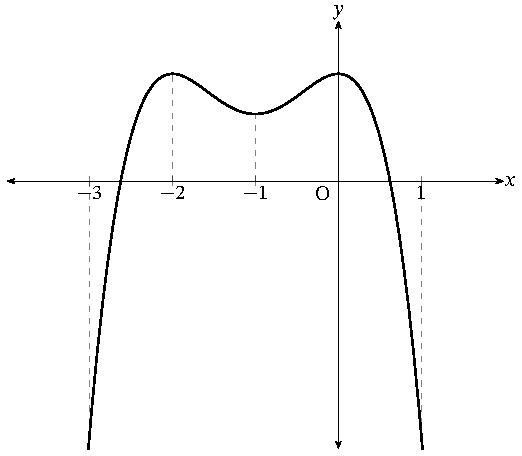
\includegraphics[keepaspectratio]{../../../../../../../figures/toan-thpt/toan-12/chan-troi/sach-giao-khoa/chuong-1/bai-1/hinh-3.pdf}}

}

\caption{Hình 3}

\end{figure}%

Luận giải: Tìm đèn

Quan sát đồ thị cho ở Hình 3, ta \textbf{phỏng đoán} rằng hàm số
\(y=f(x)\) \emph{đơn điệu} trên các khoảng \((-3;-2)\), \((-2;-1)\),
\((-1;0)\), và \((0;1)\). Cụ thể:

\begin{itemize}
\tightlist
\item
  Hàm số \textbf{có vẻ} \emph{đồng biến (tăng)} trên các khoảng
  \((-3;-2)\) và \((-1;0)\), vì với \(x_1<x_2\), đồ thị cho thấy
  \(f(x_1)<f(x_2)\).
\item
  Hàm số \textbf{có vẻ} \emph{nghịch biến (giảm)} trên các khoảng
  \((-2;-1)\) và \((0;1)\), vì đồ thị cho thấy \(f(x_1)>f(x_2)\) với
  \(x_1<x_2\).
\end{itemize}

Lưu ý rằng đây chỉ là những nhận xét dựa trên trực quan từ đồ thị, không
phải kết luận được kiểm chứng từ công thức hàm số.

Tóm lại, các khoảng đơn điệu trên chỉ mang tính phỏng đoán. Để khẳng
định chính xác tính đồng biến hay nghịch biến theo định nghĩa toán học,
cần biết công thức của hàm số và kiểm tra bằng định nghĩa hoặc đạo hàm
nếu có.

\marginnote{\begin{footnotesize}

\begin{tcolorbox}[enhanced jigsaw, arc=.35mm, colback=white, bottomrule=.15mm, toptitle=1mm, left=2mm, breakable, colbacktitle=quarto-callout-note-color!10!white, rightrule=.15mm, titlerule=0mm, leftrule=.75mm, bottomtitle=1mm, title={Ghi chú}, coltitle=black, colframe=quarto-callout-note-color-frame, toprule=.15mm, opacitybacktitle=0.6, opacityback=0]

Trong bài toán này, học sinh được yêu cầu xác định các khoảng đồng biến
- nghịch biến từ đồ thị mà không có công thức hàm số. Việc sử dụng cụm
từ ``có vẻ đồng biến'' hay ``được phỏng đoán là nghịch biến'' giúp học
sinh nhận diện tính đơn điệu thông qua trực quan, nhưng vẫn giữ thái độ
thận trọng về mặt lập luận toán học.

Điều này giúp tránh hiểu lầm phổ biến rằng: ``nhìn thấy đồ thị đi lên
thì hàm chắc chắn đồng biến''. Trên thực tế, để kết luận một cách chính
xác, học sinh cần sử dụng định nghĩa hoặc đạo hàm khi có công thức.

Khuyến khích giáo viên đặt thêm câu hỏi mở rộng như:

\begin{itemize}
\tightlist
\item
  Nếu đồ thị có đoạn gãy khúc thì sao?
\item
  Liệu có cần hàm liên tục mới nói đến đơn điệu?
\item
  Nếu chỉ xét đạo hàm âm/dương thì có đủ chưa?
\end{itemize}

\end{tcolorbox}

\end{footnotesize}}

Kết quả

\begin{itemize}
\tightlist
\item
  Hàm số đồng biến trên các khoảng \((-3;-2)\) và \((-1;0)\), vì đồ thị
  cho thấy \(f(x_1)<f(x_2)\) với \(x_1<x_2\) trên từng khoảng.
\item
  Hàm số nghịch biến trên các khoảng \((-2;-1)\) và \((0;1)\), vì đồ thị
  cho thấy \(f(x_1)>f(x_2)\) với \(x_1<x_2\) trên từng khoảng.
\end{itemize}

Hoạt động khám phá 1

\begin{figure}

\begin{minipage}{0.50\linewidth}
Cho hàm số \(y=f(x)=x^2\).

\begin{enumerate}
\def\labelenumi{\alph{enumi}.}
\tightlist
\item
  Từ đồ thị của hàm số \(y=f(x)\) (Hình 4), hãy chỉ ra các khoảng đồng
  biến và nghịch biến của hàm số đã cho.
\item
  Tính đạo hàm \(f'(x)\) và xét dấu \(f'(x)\).
\item
  Từ đó, nhận xét về mối liên hệ giữa các khoảng đồng biến, nghịch biến
  của hàm số với dấu của \(f'(x)\).
\end{enumerate}

\end{minipage}%
%
\begin{minipage}{0.50\linewidth}

\begin{figure}[H]

{\centering \pandocbounded{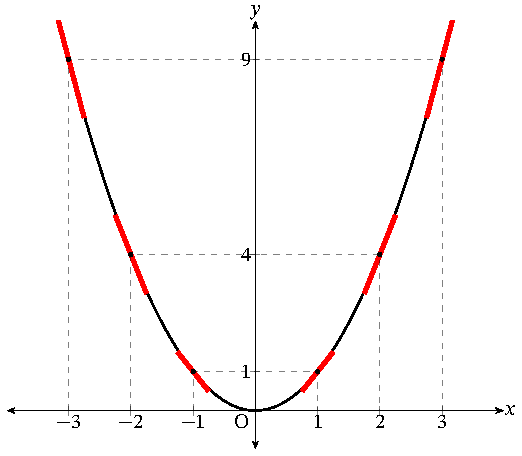
\includegraphics[keepaspectratio]{../../../../../../../figures/toan-thpt/toan-12/chan-troi/sach-giao-khoa/chuong-1/bai-1/hinh-4.pdf}}

}

\subcaption{Hình 4}

\end{figure}%

\end{minipage}%

\end{figure}%

Luận giải

\begin{enumerate}
\def\labelenumi{\alph{enumi}.}
\item
  Quan sát đồ thị ở Hình 4 cho thấy:

  \begin{itemize}
  \tightlist
  \item
    Hàm số nghịch biến trên khoảng \((-\infty;0)\), vì với mọi
    \(x_1<x_2\) trong khoảng này, đều có \(f(x_1)>f(x_2)\). Khẳng định
    này có thể kiểm bằng công thức của hàm số. Với mọi
    \(x_1,x_2\in(-\infty,0)\) và \(x_1<x_2\), theo quy tắc nhân với số
    âm, xét thấy \[
      x_1^2 > x_1\cdot x_2
     \] và \[
      x_1\cdot x_2 > x_2^2.
     \] Suy ra \(x_1^2>x_2^2\), tức là \(f(x_1)>f(x_2)\).
  \item
    Hàm số đồng biến trên khoảng \((0;+\infty)\), vì với mọi \(x_1<x_2\)
    trong khoảng này, đều có \(f(x_1)<f(x_2)\). Khẳng định này có thể
    kiểm lại bằng công thức của hàm số. Kiểm chứng tương tự bằng cách
    xét các công thức: \[
      x_1^2 < x_1\cdot x_2
     \] và \[
      x_1\cdot x_2 < x_2^2.
     \] Suy ra \(x_1^2<x_2^2\), tức là \(f(x_1)<f(x_2)\).
  \end{itemize}
\item
  Đạo hàm của \(f(x)=x^2\) là \(f'(x)=2x\).

  \begin{itemize}
  \tightlist
  \item
    Với \(x = 0\), rõ ràng \(f'(x) = 0\).
  \item
    Với mọi \(x < 0\), khi nhân \(2\) với một số âm thì
    \(f'(x) = 2x < 0\).
  \item
    Với mọi \(x > 0\), khi nhân \(2\) với một số dương thì
    \(f'(x) = 2x > 0\).
  \end{itemize}

  Có thể lập \emph{bảng xét dấu} như dưới đây để trình bày một cách trực
  quan hơn về dấu của đạo hàm.

  \begin{figure}[H]

  {\centering 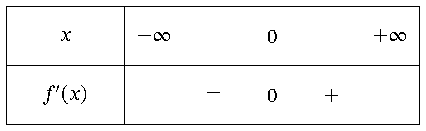
\includegraphics[width=3.64583in,height=\textheight,keepaspectratio]{../../../../../../../figures/toan-thpt/toan-12/chan-troi/sach-giao-khoa/chuong-1/bai-1/hdkp1-bang-xet-dau-dh.pdf}

  }

  \caption{Bảng xét dấu \(f'(x)=2x\).}

  \end{figure}%

  \begin{quote}
  Khi xét dấu của đạo hàm, việc đầu tiên là giải phương trình
  \(f'(x) = 0\). Vì sao? Vì nghiệm của phương trình này chính là những
  điểm mà đạo hàm chuyển dấu - hay nói cách khác, là những điểm có thể
  xảy ra sự thay đổi về chiều biến thiên. Những điểm ấy thường gắn với
  cực trị hoặc là ranh giới của khoảng đơn điệu. Không tìm chúng, tức là
  đang dò đường trong sương mù mà chưa biết ngã rẽ.
  \end{quote}
\item
  Từ kết quả xét dấu của đạo hàm, có thể thấy \(f'(x)<0\) trên khoảng
  nghịch biến và \(f'(x)>0\) trên khoảng đồng biến.
\end{enumerate}

Kết quả

\begin{enumerate}
\def\labelenumi{\alph{enumi}.}
\tightlist
\item
  Theo đồ thị Hình 4:

  \begin{itemize}
  \tightlist
  \item
    Hàm số nghịch biến trên khoảng \((-\infty;0)\).
  \item
    Hàm số đồng biến trên khoảng \((0;+\infty)\).
  \end{itemize}
\item
  Đạo hàm của \(f(x)=x^2\) là \(f'(x)=2x\).

  \begin{itemize}
  \tightlist
  \item
    Với \(x = 0\): \(f'(x) = 0\).
  \item
    Với \(x < 0\): \(f'(x) < 0\).
  \item
    Với \(x > 0\): \(f'(x) > 0\).
  \end{itemize}
\item
  Đạo hàm \(f'(x)\) âm trên khoảng nghịch biến, dương trên khoảng đồng
  biến.
\end{enumerate}

Luận giải: Tìm đèn

Kết quả

\begin{enumerate}
\def\labelenumi{\alph{enumi}.}
\tightlist
\item
  Tính đơn điệu của hàm số \(f(x)=x^3-6x^2+9x\)

  \begin{itemize}
  \tightlist
  \item
    Hàm số đồng biến trên: \((-\infty;1)\) và \((3;+\infty)\).
  \item
    Hàm số nghịch biến trên: \((1;3)\).
  \end{itemize}
\item
  Tính đơn điệu của hàm số \(g(x)=\frac{1}{x}\)

  \begin{itemize}
  \tightlist
  \item
    Hàm số nghịch biến trên: \((-\infty;0)\) và \((0;+\infty)\).
  \end{itemize}
\end{enumerate}

Thực hành 3

Chứng minh rằng hàm số \(f(x)=3x-\sin x\) đồng biến trên \(\mathbb{R}\).

Luận giải

Hàm số \(f(x) = 3x - \sin x\) xác định trên \(\mathbb{R}\) và có đạo hàm

\[
    f'(x) = 3 - \cos x.
\]

Vì \(\cos x \le 1\) với mọi \(x \in \mathbb{R}\), nên

\[
    f'(x) = 3 - \cos x \ge 3 - 1 = 2 > 0, \quad \forall x \in \mathbb{R}.
\]

Đạo hàm luôn dương trên \(\mathbb{R}\), suy ra hàm số đồng biến trên
\(\mathbb{R}\).

\begin{tcolorbox}[enhanced jigsaw, arc=.35mm, colback=white, bottomrule=.15mm, toptitle=1mm, left=2mm, breakable, colbacktitle=quarto-callout-tip-color!10!white, rightrule=.15mm, titlerule=0mm, leftrule=.75mm, bottomtitle=1mm, title={Ngách Chậm Tiêu}, coltitle=black, colframe=quarto-callout-tip-color-frame, toprule=.15mm, opacitybacktitle=0.6, opacityback=0]

Hàm số \(f(x)=3x-\sin x\) có tập xác định là \(D=\mathbb{R}\) và đạo hàm
\(f'(x)=3-\cos x\). Với mọi \(x\in\mathbb{R}\), luôn có bất đẳng thức

\[
    -1\leq \cos x\leq 1.
\]

Nhân -1 vào các vế, để có bất đẳng thức đảo chiều

\[
    1\geq -\cos x\geq -1.
\]

Cộng 3 vào các vế, để có bất đẳng thức

\[
    4\geq 3-\cos x\geq 2.
\]

Tức là \(2\leq f'(x)\leq 4\). Vậy, \(f'(x)>0\) với mọi
\(x\in \mathbb{R}\), mà tập xác định của \(f(x)\) là \(D=\mathbb{R}\),
nên suy ra \(f(x)\) đồng biến trên \(\mathbb{R}\).

\marginnote{\begin{footnotesize}

\begin{tcolorbox}[enhanced jigsaw, arc=.35mm, colback=white, bottomrule=.15mm, toptitle=1mm, left=2mm, breakable, colbacktitle=quarto-callout-note-color!10!white, rightrule=.15mm, titlerule=0mm, leftrule=.75mm, bottomtitle=1mm, title={Ghi chú}, coltitle=black, colframe=quarto-callout-note-color-frame, toprule=.15mm, opacitybacktitle=0.6, opacityback=0]

\begin{itemize}
\item
  \textbf{Vai trò của đạo hàm:} Khi muốn kiểm tra xem một hàm số có đồng
  biến hay không, đạo hàm là công cụ đáng tin cậy. Việc đạo hàm luôn
  \textbf{dương} chính là dấu hiệu rõ ràng cho tính \textbf{đồng biến}.
\item
  \textbf{Lưu ý:} Không chỉ tính đạo hàm rồi nhìn qua là kết luận. Cần
  xác định kỹ xem đạo hàm \textbf{lớn hơn, nhỏ hơn hay bằng 0} ở đâu ---
  và \textbf{luôn luôn} hay \textbf{chỉ tại vài điểm}.
\item
  \textbf{Trực giác:} Hàm số \(f(x) = 3x - \sin x\) là một hàm bậc nhất
  kết hợp với một dao động nhỏ (do \(\sin x\)). Trực giác có thể gợi ý
  nó ``tăng dần'', nhưng \textbf{chỉ có đạo hàm mới xác nhận chắc chắn}
  điều đó.
\item
  \textbf{Mở rộng:} Bản thân \(\cos x\) là hàm dao động từ -1 đến 1, nên
  \(3 - \cos x\) dao động từ \(2\) đến \(4\). Điều này cho thấy đạo hàm
  \textbf{không chỉ dương mà còn luôn lớn hơn hoặc bằng 2 và bé hơn hoặc
  bằng 4}, nên hàm số này ``tăng đều đặn'' chứ không phải chỉ là ``tăng
  nhẹ nhàng'' hay ``tăng mạnh mẽ''.

  \begin{quote}
  Hàm số này đúng kiểu ``tăng có tâm'' - không lề mề, mà cũng chẳng lăng
  xăng. Lúc nào cũng điềm đạm, bước đều như thể có ai đó bấm nhịp phía
  sau. Một bên thì lề mề như rùa mới ngủ dậy là anh \(\ln x\), một bên
  lại lăng xăng như sóc vừa uống trà đá là anh \(e^x\).
  \end{quote}
\end{itemize}

\end{tcolorbox}

\end{footnotesize}}

Vận dụng 1

Hãy trả lời câu hỏi trong Hoạt động khởi động bằng cách xét dấu đạo hàm
của hàm số \(h(t)=6t^3-81t^2+324t\) với \(0\leq t\leq 8\).

Luận giải

Đạo hàm của \(h(t)\) là \(h'(t)=18t^2-162t+324\). Để xét dấu \(h'(t)\)
với \(0\leq t\leq 8\), trước tiên, cần giải phương trình \(h'(t)=0\) với
\(0\leq t\leq 8\). Phương trình này có hai nghiệm thỏa mãn điều kiện là
\(t=3\) và \(t=6\). Bảng xét dấu đạo hàm:

\begin{figure}[H]

{\centering 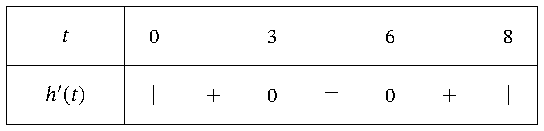
\includegraphics[width=0.6\linewidth,height=\textheight,keepaspectratio]{../../../../../../../figures/toan-thpt/toan-12/chan-troi/sach-giao-khoa/chuong-1/bai-1/vd1-bang-xet-dau-dh.pdf}

}

\caption{Bảng xét dấu \(h'(t)\).}

\end{figure}%

\begin{itemize}
\tightlist
\item
  Khinh khí cầu \emph{tăng} độ cao trong các khoảng \((0;3)\) và
  \((6;8)\).
\item
  Khinh khí cầu \emph{giảm} độ cao trong khoảng \((3;6)\).
\item
  Tại \(t=3\) phút, đ\emph{ạo hàm đổi dấu từ dương sang âm}. Điều này có
  nghĩa là độ cao tại thời điểm 3 phút là lớn nhất so với các thời điểm
  xung quanh, ít nhất là với tất cả \(t\in(0;6)\backslash\{3\}\).
\item
  Tại \(t=6\) phút, \emph{đạo hàm đổi dấu từ âm sang dương}. Điều này có
  nghĩa là độ cao tại thời điểm 6 phút là nhỏ nhất so với các thời điểm
  xung quanh, ít nhất là với tất cả \(t\in(3;8)\backslash\{6\}\).
\end{itemize}

Hoạt động khám phá 2

Luận giải

Hãy quan sát đồ thị hàm số \(y = f(x) = x^3 - 3x^2 + 1\) trong Hình 5.

\begin{enumerate}
\def\labelenumi{\alph{enumi}.}
\item
  Tại điểm \(x = 0\), đồ thị vươn lên một đỉnh rõ rệt. Khi rời khỏi điểm
  này một khoảng nhỏ về cả hai phía, giá trị của hàm số đều nhỏ hơn giá
  trị tại chính điểm đó. Điều này cho thấy có thể chọn một khoảng
  \((a; b)\) bao quanh \(x = 0\) sao cho với mọi \(x \ne 0\) trong
  khoảng này, luôn có \(f(x) < f(0)\). Có vô số khoảng như vậy, miễn là
  khoảng được chọn đủ nhỏ để hoàn toàn nằm trong vùng mà giá trị của hàm
  số không vượt lên trên \(f(0)\). Ví dụ, \((-1;1)\) và
  \(\left(-2;\frac{1}{2}\right)\).
\item
  Tại điểm \(x = 2\), đồ thị chạm đến một vùng trũng rõ rệt. Nếu xét các
  điểm lân cận ở hai phía, giá trị của hàm số đều lớn hơn giá trị tại
  \(x = 2\). Do đó, có thể chọn một khoảng \((a; b)\) chứa điểm này sao
  cho với mọi \(x \ne 2\) trong khoảng, luôn có \(f(x) > f(2)\). Tương
  tự như ở câu a, cũng có vô số khoảng thỏa mãn điều kiện. Ví dụ,
  \((1;3)\) và \(\left(\frac{3}{2};4\right)\).
\item
  Hai điểm \(x=0\) và \(x=2\) vừa xét đều cho thấy một tính chất đặc
  biệt: có thể tìm được những khoảng bao quanh mỗi điểm sao cho trong
  khoảng ấy, giá trị của hàm số tại chính điểm đó đều \emph{vượt trội}
  so với các điểm còn lại - một bên là cao nhất khoảng, một bên là tháp
  nhất khoảng.

  Điều này đặt ra một câu hỏi tự nhiên: liệu những điểm khác trên đồ
  thị, như \(x=1\), có chia sẻ đặc điểm tương tự, hay đó chính là các
  điểm đặc biệt của hàm số này? Đây chính là cách diễn đạt khác cho câu
  hỏi c.

  Quan sát đồ thị cho thấy, tính chất ấy không còn xuất hiện ở đây. Phía
  bên trái \(x = 1\), đồ thị đang đi xuống, tức là hàm số giảm và có giá
  trị lớn hơn \(f(1)\). Phía bên phải, đồ thị tiếp tục hạ thấp hơn nữa,
  tức là giá trị hàm số nhỏ hơn \(f(1)\). Nói cách khác, trong bất kỳ
  khoảng nào chứa \(x = 1\), đều tồn tại điểm có giá trị lớn hơn và điểm
  có giá trị nhỏ hơn so với \(f(1)\). Không thể tìm được một khoảng nào
  mà trong đó \(f(1)\) vượt trội theo bất kỳ chiều nào như đã thấy tại
  hai điểm trước.
\end{enumerate}

Kết quả

\begin{enumerate}
\def\labelenumi{\alph{enumi}.}
\item
  Có vô số khoảng \((a;b)\) thỏa yêu cầu: dễ thấy như \((-1;1)\),
  \((-1;2)\); hoặc chưa được thể hiện rõ trên hình như
  \((-1;\frac{1}{2})\), \((-\frac{1}{2};1)\), \((-\frac{1}{2};2)\),
  \((-2;1)\), \((-2;2)\), v.v.. Các khoảng được chọn miễn sao đủ nhỏ để
  giá trị tại \(x=0\) vẫn luôn lớn nhất trong khoảng đó.
\item
  Tương tự, cũng có vô số khoảng \((a;b)\) thỏa yêu cầu: \((-1;3)\),
  \((0;3)\), \((1;3)\), \((-\frac{1}{2};3)\), \((\frac{1}{2};3)\),
  \((\frac{3}{2};3)\), \((-2;3)\), \((-2;\frac{5}{2})\), \((-2;4)\),
  v.v.. Các khoảng được chọn càng rộng thì càng cần kiểm tra cẩn thận để
  đảm bảo không có điểm nào trong khoảng đó cho giá trị nhỏ hơn
  \(f(2)\).
\item
  Không tồn tại khoảng \((a;b)\) thỏa yêu cầu, vì trong bất kỳ khoảng
  nào chứa \(x=1\), đều có điểm cho giá trị hàm số lớn hơn và điểm cho
  giá trị nhỏ hơn so với \(f(1)\).
\end{enumerate}

Thực hành 4

Tìm các điểm cực trị của hàm số \(y=f(x)\) có đồ thị cho ở Hình 8.

\begin{figure}[H]

{\centering \pandocbounded{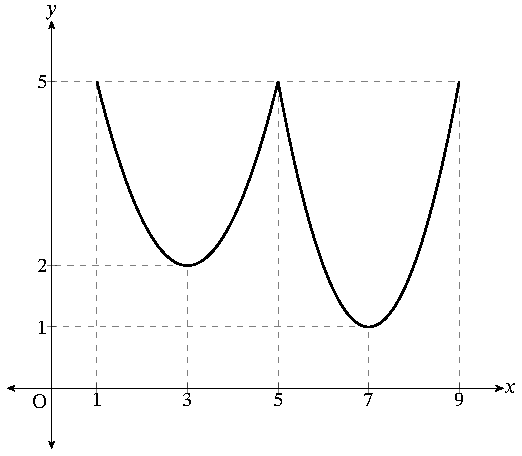
\includegraphics[keepaspectratio]{../../../../../../../figures/toan-thpt/toan-12/chan-troi/sach-giao-khoa/chuong-1/bai-1/hinh-8.pdf}}

}

\caption{Hình 8}

\end{figure}%

Luận giải

Đồ thị của hàm số \(y=f(x)\) ở Hình 8 có 3 điểm cực trị, hai điểm cực
tiểu là \((3;2)\) và \((7;1)\), cùng một điểm cực đại là \((5;5)\).

\begin{itemize}
\tightlist
\item
  Điểm \((3;2)\) là một điểm cực tiểu vì tồn tại khoảng \((2;4)\) thỏa
  mãn \(f(x)>f(3)=2\) với mọi \(x\in(2;4)\backslash\{3\}\). Điểm
  \((7;1)\) cũng là điểm cực tiểu với lý do tương tự.\\
\item
  Điểm \((5;5)\) là một điểm cực đại vì tồn tại khoảng \((4;6)\) thỏa
  mãn \(f(x)>f(5)=5\) với mọi \(x\in(4;6)\backslash\{5\}\).
\end{itemize}

\begin{tcolorbox}[enhanced jigsaw, arc=.35mm, colback=white, bottomrule=.15mm, toptitle=1mm, left=2mm, breakable, colbacktitle=quarto-callout-tip-color!10!white, rightrule=.15mm, titlerule=0mm, leftrule=.75mm, bottomtitle=1mm, title={Ngách Mộng Du}, coltitle=black, colframe=quarto-callout-tip-color-frame, toprule=.15mm, opacitybacktitle=0.6, opacityback=0]

Trên một sân khấu trải dài từ 1 đến 9, đồ thị lần lượt đưa ba ngôi sao
bước ra trong ánh đèn rực rỡ.

Ở điểm \(x=3\), đồ thị nhẹ nhàng cúi mình, tao nên một cực tiểu dịu
dàng. Từ 2 đến 4, mọi điểm trong ấy đều cao hơn, như thể khán giả đồng
loạt cuối đầu nhìn vào chỗ nhân vật chính bước ra.

Xa hơn, tại \(x=7\), lại một pha cuối mình mềm mại, lần này càng khiêm
tốn hơn, chạm đến giá trị thấp nhất là 1. Hãy xem, trong vùng từ 6 đến
8, mọi giá trị khác đều cao hơn, như cả khán phòng lặng yên để lắng nghe
một nốt trầm tuyệt đẹo. Cực tiểu lần hai, lay động lòng người.

Và rồi, ở giữa hai kẻ ấy, tại \(x=5\), đồ thị bất ngờ vươn lên đầy kiêu
hãnh. Khắp vùng từ \(4\) đến \(6\), không ai sánh bằng. Đây chưa phải là
nơi cao nhất dưới trời \([1;9]\) nhưng chắc chắn là điểm rực rỡ nhất,
mọi ánh đèn sân khấu muốn dồn lại - một điểm cực đại, chói sáng và tự
tin như một đỉnh núi vươn mình chạm đến trời cao.

Hai cực tiểu dịu dàng, một cực đại bừng sáng. Ba điểm cực trị ấy không
chỉ tạo hình cho đồ thị, mà còn kể một câu chuyện đẹp - bằng chính sự
lên xuống của hàm số.

\end{tcolorbox}

Kết quả

Đồ thị của hàm số \(y=f(x)\) ở Hình 8 có 3 điểm cực trị. Cụ thể:

\begin{itemize}
\tightlist
\item
  Cực tiểu: \((3;2)\) và \((7;1)\),
\item
  Cực đại: \((5;5)\).
\end{itemize}

Hoạt động khám phá 3

Thực hành 5

Tìm cực trị của hàm số \(g(x)=\frac{x^2+x+4}{x+1}\).

Vận dụng 2

Một phần lát cắt của dãy núi có độ cao tính bằng mét được mô tả bởi hàm
số

\[
    y=h(x)=-\frac{1}{1320000}x^3+\frac{9}{3520}x^2-\frac{81}{44}x+840 \text{ với } 0\leq x\leq 2000.
\]

Tìm toạ độ các đỉnh của lát cắt dãy núi trên đoạn \([0; 2 000]\).

\begin{figure}[H]

{\centering \pandocbounded{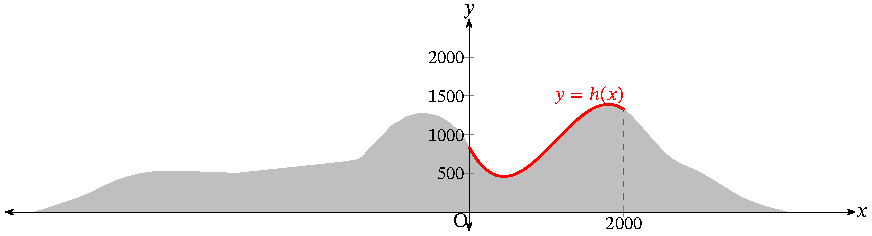
\includegraphics[keepaspectratio]{../../../../../../../figures/toan-thpt/toan-12/chan-troi/sach-giao-khoa/chuong-1/bai-1/hinh-10.pdf}}

}

\caption{Hình 10 (\emph{Theo:} Tập bản đồ bài tập và bài thực hành Địa
lí 8, Nhà xuất bản Giáo dục Việt Nam, 2011)}

\end{figure}%

\subsection{Bài tập}\label{buxe0i-tux1eadp}

Bài tập 1

Tìm các khoảng đơn điệu và cực trị của các hàm số có đồ thị cho ở Hình
11.

Bài tập 2

Xét tính đơn điệu và tìm điểm cực trị của các hàm số sau:

\begin{figure}

\begin{minipage}{0.33\linewidth}

\begin{enumerate}
\def\labelenumi{\alph{enumi}.}
\tightlist
\item
  \(y=4x^3+3x^2-36x+6\)
\end{enumerate}

\end{minipage}%
%
\begin{minipage}{0.33\linewidth}

\begin{enumerate}
\def\labelenumi{\alph{enumi}.}
\setcounter{enumi}{1}
\tightlist
\item
  \(y=\frac{x^2-2x-7}{x-4}\)
\end{enumerate}

\end{minipage}%

\end{figure}%

Bài tập 3

Tìm cực trị của các hàm số sau:

\begin{figure}

\begin{minipage}{0.33\linewidth}

\begin{enumerate}
\def\labelenumi{\alph{enumi}.}
\tightlist
\item
  \(y=2x^3+3x^2-36x+1\)
\end{enumerate}

\end{minipage}%
%
\begin{minipage}{0.33\linewidth}

\begin{enumerate}
\def\labelenumi{\alph{enumi}.}
\setcounter{enumi}{1}
\tightlist
\item
  \(y=\frac{x^2-8x+10}{x-2}\)
\end{enumerate}

\end{minipage}%
%
\begin{minipage}{0.33\linewidth}

\begin{enumerate}
\def\labelenumi{\alph{enumi}.}
\setcounter{enumi}{2}
\tightlist
\item
  \(y=\sqrt{-x^2+4}\)
\end{enumerate}

\end{minipage}%

\end{figure}%

Lời giải

Bài tập 4

Chứng minh rằng hàm số \(y=\frac{2x+1}{x-3}\) nghịch biến trên từng
khoảng xác định của nó.

Lời giải

Bài tập 5

Kim ngạch xuất khẩu rau quả của Việt Nam trong các năm từ 2010 đến 2017
có thể được tính xấp xỉ bằng công thức
\(f(x)=0,01x^3–0,04x^2+0,25x + 0,44\) (tỉ USD) với \(x\) là số năm tính
từ 2010 đến 2017 (\(0 \leq x \leq 7\)).

(\emph{Theo}: https://infographics.vn/interactive-xuat-khau-rau-quadu-
bao-bung-no-dat-4-ty-usd-trong-nam-2023/116220.vna)

\begin{enumerate}
\def\labelenumi{\alph{enumi}.}
\tightlist
\item
  Tính đạo hàm của hàm số \(y=f(x)\).
\item
  Chứng minh rằng kim ngạch xuất khẩu rau quả của Việt Nam tăng liên tục
  trong các năm từ 2010 đến 2017.
\end{enumerate}

Lời giải

Bài tập 7

Xét một chất điểm chuyển động dọc theo trục Ox. Toạ độ của chất điểm tại
thời điểm \(t\) được xác định bởi hàm số \(x(t) = t^3 – 6t^2 + 9t\) với
\(t \geq 0\). Khi đó \(x'(t)\) là vận tốc của chất điểm tại thời điểm
\(t\), kí hiệu \(v(t)\); \(v'(t)\) là gia tốc chuyển động của chất điểm
tại thời điểm \(t\), kí hiệu \(a(t)\).

\begin{enumerate}
\def\labelenumi{\alph{enumi}.}
\tightlist
\item
  Tìm các hàm \(v(t)\) và \(a(t)\).
\item
  Trong khoảng thời gian nào vận tốc của chất điểm tăng, trong khoảng
  thời gian nào vận tốc của chất điểm giảm?
\end{enumerate}

Lời giải

Bài tập 8

Đạo hàm \(f'(x)\) của hàm số \(y=f(x)\) có đồ thị như Hình 12. Xét tính
đơn điệu và tìm điểm cực trị của hàm số \(y=f(x)\).

\begin{figure}[H]

{\centering \pandocbounded{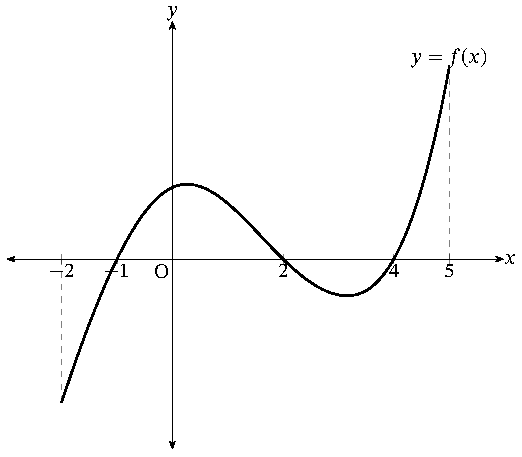
\includegraphics[keepaspectratio]{../../../../../../../figures/toan-thpt/toan-12/chan-troi/sach-giao-khoa/chuong-1/bai-1/hinh-12.pdf}}

}

\caption{Hình 12}

\end{figure}%

Luận giải

\end{tcolorbox}




\end{document}
